
\documentclass[aspectratio=43]{beamer}
% Theme works only with a 4:3 aspect ratio
\usetheme{CSCS}

\usepackage{tikz}
\usepackage{pgfplots}
\usepackage{pgfplotstable}
\usetikzlibrary{pgfplots.groupplots,spy}
\usepackage{listings}
\usepackage{color}
\usepackage{tcolorbox}
\usepackage{anyfontsize}
\usepackage{xspace}

% define footer text
\newcommand{\footlinetext}{CUDA Introduction}

% Select the image for the title page
\newcommand{\picturetitle}{cscs_images/image5.pdf}

% fonts for maths
\usefonttheme{professionalfonts}
\usefonttheme{serif}

% source code listing
\newcommand{\axpy}{{\ttfamily axpy}\xspace}
\newcommand{\extra}{{\bfseries extra}:\xspace}
\newcommand{\lst}[1]{\colorbox{white!90!blue}{\lstinline!#1!}}
\newcommand{\lstfont}[1]{\color{#1}\scriptsize\ttfamily}
\newcommand{\lsttinyfont}[1]{\color{#1}\fontsize{7}{7}\ttfamily}
\newcommand{\lstinlinefont}[1]{\color{#1}\scriptsize\ttfamily}

\lstset{
    language=[ANSI]C++,
    basicstyle=\lstinlinefont{blue!30!black},
    breaklines=true
}

\definecolor{codenumber}{rgb}{0.5,0.5,0.5}
\definecolor{codekeyword}{rgb}{0.9,0.4,0.7}
\definecolor{codeCUDA}{rgb}{1.0,0.6,0.6}

\lstdefinestyle{boxcuda}{
    language=[ANSI]C++,
    showstringspaces=false,
    backgroundcolor=\color{white!10!black},
    basicstyle=\lstfont{white},
    identifierstyle=\lstfont{white},
    keywordstyle=\lstfont{magenta!40!white},
    numberstyle=\lstfont{white},
    stringstyle=\lstfont{cyan},
    commentstyle=\lstfont{yellow!30!white},
    emph={
        cudaMemcpy,
        cudaMalloc,
        cudaFree,
        cudaMemcpyHostToDevice,
        cudaMemcpyDeviceToHost,
        cudaSuccess,
        cudaGetLastError,
        cudaGetErrorString,
        cudaErrorMemoryAllocation,
        cudaError_t,
        __global__, __shared__, __device__, __host__,
        threadIdx, blockIdx, blockDim, gridDim,
    },
    emphstyle={\lstfont{green!60!white}},
    breaklines=true
}

\lstdefinestyle{boxcudatiny}{
    language=[ANSI]C++,
    showstringspaces=false,
    backgroundcolor=\color{white!10!black},
    basicstyle=\lsttinyfont{white},
    identifierstyle=\lsttinyfont{white},
    keywordstyle=\lsttinyfont{magenta!40!white},
    numberstyle=\lsttinyfont{white},
    stringstyle=\lsttinyfont{cyan},
    commentstyle=\lsttinyfont{yellow!30!white},
    emph={
        cudaMemcpy,
        cudaMalloc,
        cudaFree,
        cudaMemcpyHostToDevice,
        cudaMemcpyDeviceToHost,
        cudaSuccess,
        cudaGetLastError,
        cudaGetErrorString,
        cudaErrorMemoryAllocation,
        cudaError_t,
        __global__, __shared__, __device__, __host__,
        threadIdx, blockIdx, blockDim, gridDim,
    },
    emphstyle={\lstfont{green!60!white}},
    breaklines=true
}

\DeclareTextFontCommand{\emph}{\bfseries}

% Please use the predifined colors:
% cscsred, cscsgrey, cscsgreen, cscsblue, cscsbrown, cscspurple, cscsyellow, cscsblack, cscswhite

\author{Ben Cumming, CSCS}
\title{Introduction to CUDA}
\subtitle{Summer School 2015}
\date{\today}

\begin{document}

% TITLE SLIDE
\cscstitle

% TABLE OF CONTENT SLIDE
% All options for table of contents:
% currentsection, currentsubsection, firstsection=xx, hideallsubsections, hideothersubsections, part=xx, pausesections, pausesubsections, sections=xx, sections={xx-yy}, sections={xx,yy}
%\cscstableofcontents[hideallsubsections]{Title}

% CHAPTER SLIDE
\cscschapter{Introduction}

%%%%
\begin{frame}[fragile]{Introduction to CUDA}
    \begin{info}{The plan}
        \begin{itemize}
            \item learn about the GPU programming model
            \item implement CUDA kernels for simple linear algebra
            \item learn how to orchestrate asynchronous computaion and communication on GPU
            \item a 2D stencil application
        \end{itemize}
    \end{info}

    \begin{info}{Prerequisites}
        \begin{itemize}
            \item I assume C++ knowledge
            \begin{itemize}
                \item I will be using C++11 (the bits that make C++ easier!)
                \item Fortran users consider working with a C++ user
            \end{itemize}
            \item No GPU or graphics experience required
        \end{itemize}
    \end{info}

\end{frame}

%%%%
\begin{frame}[fragile]{What is CUDA?}
    \begin{info}{A superset of C++}
        \begin{itemize}
            \item write CPU code using C++ (C++11 since CUDA 6.5)
            \item write kernels to run on GPU using new keywords
            \item provides special syntax for launching kernels on GPU
        \end{itemize}
    \end{info}

    \begin{info}{GPU specific}
        \begin{itemize}
            \item the CUDA extensions define the \emph{programming model}
            \item PRO : programming model is well suited to GPU
            \item CON : GPU-specific
        \end{itemize}
    \end{info}

    \begin{info}{Extras}
        \begin{itemize}
            \item provides library/API
            \item tools for profiling and debugging
        \end{itemize}
    \end{info}
\end{frame}

%%%%
\begin{frame}[fragile]{Device and Host Memory}
    \begin{center}
        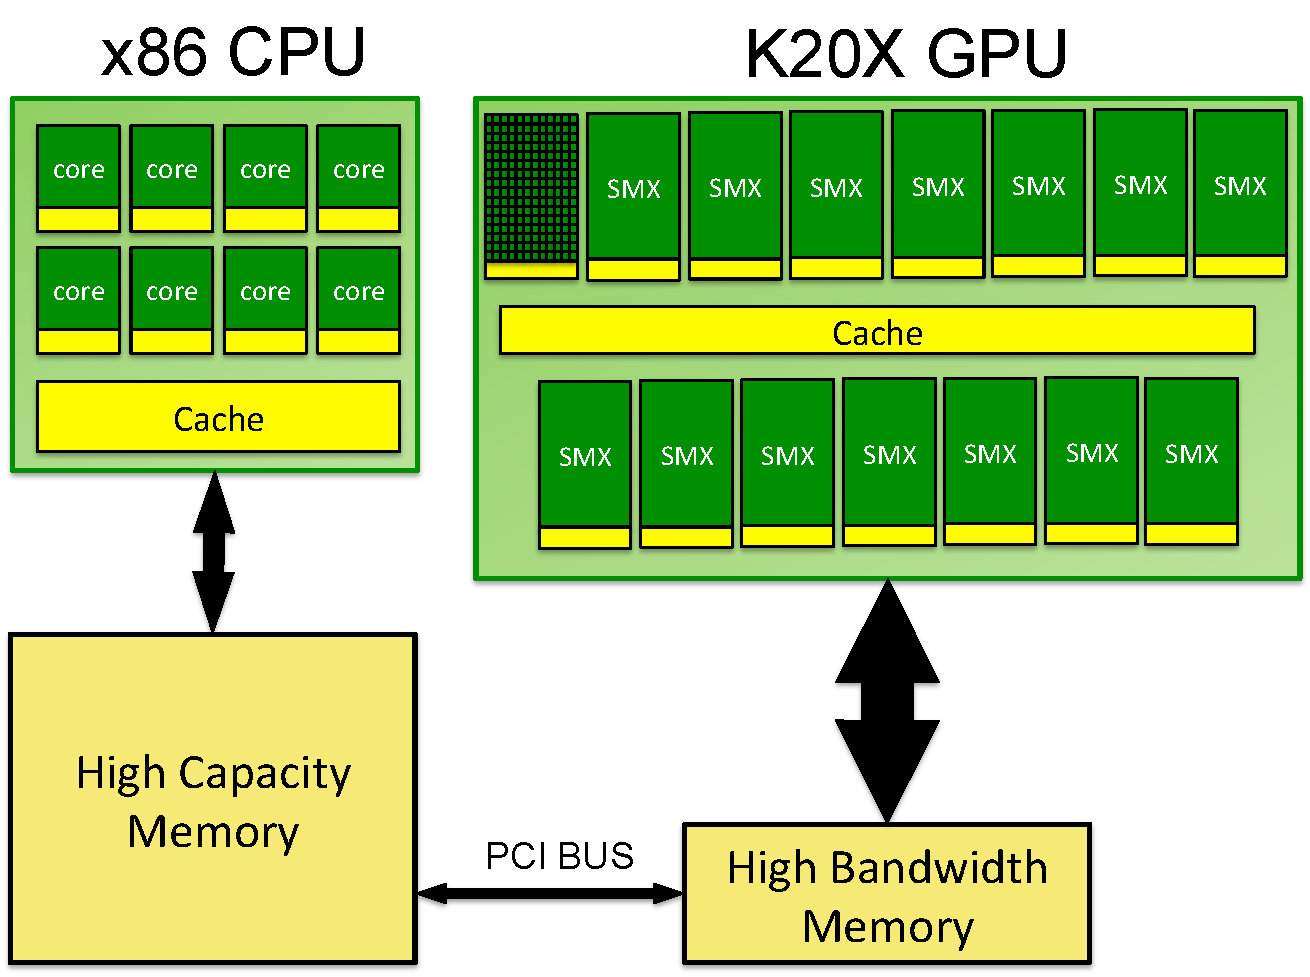
\includegraphics[width=0.9\textwidth]{./images/node.pdf}
    \end{center}
\end{frame}

%%%%
\begin{frame}[fragile]{Device and Host Memory}
    \begin{info}{host and device have separate memory spaces}
        \begin{itemize}
            \item data must be copied between host and device memory via PCI
            \item data must be in device memory for kernels to access
            \item ensure data is in the right memory space \emph{before} computation starts
                \begin{itemize}
                    \item PCIe2 = 6-12 GB/s
                    \item CPU socket = 35-50 GB/s
                    \item K20X  = 180 GB/s
                \end{itemize}
        \end{itemize}
    \end{info}

    \begin{info}{CUDA uses C pointers to reference GPU memory}
        \begin{itemize}
            \item it isn't possible to tell whether a pointer points to device or host
            \item accessing a device pointer in host code is \emph{undefined behaviour}
        \end{itemize}
    \end{info}

\end{frame}

%%%%
\begin{frame}[fragile]{Allocating Memory}

    \begin{info}{allocating memory on device}
        \centering \lst{cudaMalloc(void **ptr, size_t size)}
    \begin{itemize}
        \item \lst{size} number of bytes to allocate
        \item \lst{ptr} points to allocated memory on exit
    \end{itemize}
    \end{info}

    \begin{info}{freeing memory on device}
        \centering \lst{cudaFree(void *ptr)}
    \end{info}

    \begin{code}{allocate 100 doubles on device}
%..................................
        \begin{lstlisting}[style=boxcuda]
double *v;
int size_in_bytes = 100*sizeof(double);
cudaMalloc(&v, size_in_bytes); // allocate memory
cudaFree(v);                   // free memory
\end{lstlisting}
%..................................
    \end{code}
\end{frame}

%%%%
\begin{frame}[fragile]{Copying data}

    \begin{info}{perform blocking copy (host waits for copy to finish)}
        \centering \lst{cudaMemcpy(void *dst, void *src, size_t size, cudaMemcpyKind kind)}
    \begin{itemize}
        \item \lst{dst} destination pointer
        \item \lst{src} source pointer
        \item \lst{size} number of \emph{bytes} to copy to \lst{dst}
        \item \lst{kind} enumerated type specifying \emph{direction} of copy:
            \lst{cudaMemcpyHostToDevice}, also \lst{DeviceToHost}, \lst{DeviceToDevice}
    \end{itemize}
    \end{info}

    \begin{code}{copy 100 doubles to device, then back to host}
%..................................
        \begin{lstlisting}[style=boxcuda]
int size = 100*sizeof(double); // size in bytes
double *v_d;
cudaMalloc(&v_d, size);
double *v_h = (double*)malloc(size);
cudaMemcpy(v_d, v_h, size, cudaMemcpyHostToDevice);
cudaMemcpy(v_h, v_d, size, cudaMemcpyDeviceToHost);
\end{lstlisting}
%..................................
    \end{code}
\end{frame}

%%%%
\begin{frame}[fragile]{Error handling}

    \begin{info}{}
        All API functions return error codes that indicate either:
        \begin{itemize}
            \item an error in the API call
            \item an error in an earlier asynchronous call
        \end{itemize}
        The return value is the enum type \lst{cudaError_t}
        \begin{itemize}
            \item e.g. \lst{cudaError_t status = cudaMalloc(&v, 100);}
            \begin{itemize}
                \item status is \{\lst{cudaSuccess}, \lst{cudaErrorMemoryAllocation}\}
            \end{itemize}
        \end{itemize}
    \end{info}

    \begin{info}{Handling errors}
        \centering \lst{const char* cudaGetErrorString(status)}
        \begin{itemize}
            \item returns a string describing status
        \end{itemize}
        \centering \lst{cudaError_t cudaGetLastError()}
        \begin{itemize}
            \item returns the last error
            \item resets status to \lst{cudaSuccess}
        \end{itemize}
    \end{info}

\end{frame}

%%%%
\begin{frame}[fragile]{Error handling}

    \begin{code}{copy 100 doubles to device, with error checking}
%..................................
        \begin{lstlisting}[style=boxcuda]
double *v_d;
int size = sizeof(double)*100;
double *v_host = (double*)malloc(size);
cudaError_t status = cudaMalloc(&v_d, size);
if(status != cudaSuccess) {
  printf("cuda error : %s\n", cudaGetErrorString(status));
  exit(1);
}
status =
  cudaMemcpy(v_d, v_h, size, cudaMemcpyHostToDevice);
if(status != cudaSuccess) {
  printf("cuda error : %s\n", cudaGetErrorString(status));
  printf("cuda error : %s\n", cudaGetErrorString(status));
  exit(1);
}
        \end{lstlisting}
%..................................
    \end{code}

    It is essential to test for errors
    \begin{itemize}
        \item but it gets tedious...
    \end{itemize}
\end{frame}

%%%%%%%%%%%%%%%%%%%%%%%%%%%%%%%%%%%%%%%%%%%%
\begin{frame}[fragile]{Exercise: API Basics}
%%%%%%%%%%%%%%%%%%%%%%%%%%%%%%%%%%%%%%%%%%%%
    Open \lst{cuda/exercises/util.h}
    \begin{enumerate}
        \item what does \lst{cude_check_error()} do?

        \item Write a template wrapper around cudaMalloc to simplify allocating memory
        \begin{itemize}
            \item use the example for \lst{malloc_host} that is already implemented
            \item remember to check for errors API errors.
            \item what are the benefits over using \lst{cudaMalloc} directly?
            \item do we need to write a similar function for \lst{cudaFree}?
        \end{itemize}

        \item Write a wrapper around \lst{cudaMemcpy} for copying data from host to device
        \begin{itemize}
            \item use the example for the reverse operation \lst{copy_device_to_host_sync}
        \end{itemize}

        \item Compile the test and run
        \begin{itemize}
            \item it will pass with no errors on success
        \end{itemize}
    \end{enumerate}

\end{frame}

% CHAPTER SLIDE
\cscschapter{Going Parallel : Kernels}

%%%%%%%%%%%%%%%%%%%%%%%%%%%%%%%%%%%%%%%%%%%%
\begin{frame}[fragile]{The CUDA Programming Model}
%%%%%%%%%%%%%%%%%%%%%%%%%%%%%%%%%%%%%%%%%%%%
    \begin{info}{threads and kernels}
        \begin{itemize}
            \item \textbf{thread} are run simultaneously on GPU (1000s)
            \item \textbf{kernel} is the task run by each thread
            \item CUDA provides the means for
            \begin{itemize}
                \item writing kernels
                \item launching many threads to execute parallel kernel
            \end{itemize}
            \begin{itemize}
                \item it hides the low-level scheduling
            \end{itemize}
        \end{itemize}
    \end{info}
    \begin{info}{Porting to CUDA}
        \begin{enumerate}
            \item formulate algorithm in terms of parallel work items
            \item write a cuda kernel which implements a work item
            \item launch the kernel on as many threads as required
        \end{enumerate}
    \end{info}

\end{frame}

%%%%%%%%%%%%%%%%%%%%%%%%%%%%%%%%%%%%%%%%%%%%
\begin{frame}[fragile]{Scaled Vector Addition (\axpy)}
%%%%%%%%%%%%%%%%%%%%%%%%%%%%%%%%%%%%%%%%%%%%
    \begin{info}{}
        The exercises use CUBLAS to perform scaled vector addition
            \vspace{-10pt}
            $$y = y + \alpha x$$
            \vspace{-25pt}
        \begin{itemize}
            \item $x$ and $y$ are vectors of length $n$
            \item $\alpha$ is scalar
        \end{itemize}
    \end{info}

    \begin{code}{\axpy implemented with for loop}
%..................................
        \begin{lstlisting}[style=boxcuda]
void axpy(double *y, double *x, double a, int n) {
  for(int i=0; i<n; ++i)
    y[i] = y[i] + a*x[i];
}
        \end{lstlisting}
%..................................
    \end{code}

    \begin{info}{}
        \axpy can be expressed into $n$ independent operations
        $$y_i \leftarrow y_i + a*x_i,\quad i = {0, 1, \dots, n-1}$$
        which can be performed independently and in any order
    \end{info}

\end{frame}

%%%%%%%%%%%%%%%%%%%%%%%%%%%%%%%%%%%%%%%%%%%%
\begin{frame}[fragile]{Writing A Kernel}
%%%%%%%%%%%%%%%%%%%%%%%%%%%%%%%%%%%%%%%%%%%%
    \begin{info}{What is a kernel?}
    \begin{itemize}
        \item a kernel defines the work item for a single thread
        \item the work is performed by many threads executing the same kernel \emph{simultaneously}
        \item Conceptually corresponds to the inner part of a loop for BLAS1 operations like \axpy
    \end{itemize}
    \end{info}

    \vspace{-10pt}
    \begin{columns}[T]
        \begin{column}{0.5\textwidth}
            \begin{codecolumn}{host : add two vectors}
%..................................
        \begin{lstlisting}[style=boxcudatiny]

void add(int *a, int *b, int n) {
  for(int i=0; i<n; ++i)
    a[i] += b[i];
}
        \end{lstlisting}
%..................................
            \end{codecolumn}
        \end{column}
        \begin{column}{0.5\textwidth}
            \begin{codecolumn}{CUDA : add two vectors}
%..................................
        \begin{lstlisting}[style=boxcudatiny]
__global__
void add(int *a, int *b, int n) {
  int i = threadIdx.x;
  a[i] += b[i];
}
        \end{lstlisting}
%..................................
            \end{codecolumn}
        \end{column}
    \end{columns}

    \vspace{-2pt}
    \begin{info}{}
    \begin{itemize}
        \item \lst{__global__} keyword indicates a kernel that called from the host
        \item \lst{ThreadIdx} used to find unique id of each thread
    \end{itemize}
    \end{info}
\end{frame}

%%%%%%%%%%%%%%%%%%%%%%%%%%%%%%%%%%%%%%%%%%%%
\begin{frame}[fragile]{Launching a Kernel}
%%%%%%%%%%%%%%%%%%%%%%%%%%%%%%%%%%%%%%%%%%%%
    \begin{info}{launching a kernel}
    \begin{itemize}
        \item host code launches a kernel on the GPU \emph{asyncronously}
        \item CUDA provides special \lst{<<<_,_>>>} syntax for launching a kernel
        \begin{itemize}
            \item \lst{foo<<<1, num_threads>>>(args... )} will launch the kernel \lst{foo} with \lst{num_threads} parallel threads.
        \end{itemize}
    \end{itemize}
    \end{info}

    \begin{columns}[T]
        \begin{column}{0.5\textwidth}
            \begin{code}{host : add two vectors}
%..................................
        \begin{lstlisting}[style=boxcuda]
const int n = 1024;
int *a, *b;
a = host_malloc<int>(n);
b = host_malloc<int>(n);
add(a, b, n);
        \end{lstlisting}
%..................................
            \end{code}
        \end{column} \begin{column}{0.5\textwidth}
            \begin{code}{CUDA : add two vectors}
%..................................
        \begin{lstlisting}[style=boxcuda]
const int n = 1024;
int *a , *b;
a = device_malloc<int>(n);
b = device_malloc<int>(n);
add<<<1,n>>>(a, b, n);
        \end{lstlisting}
%..................................
            \end{code}
        \end{column}
    \end{columns}

\end{frame}

%%%%%%%%%%%%%%%%%%%%%%%%%%%%%%%%%%%%%%%%%%%%
\begin{frame}[fragile]{Exercise: My First Kernel}
%%%%%%%%%%%%%%%%%%%%%%%%%%%%%%%%%%%%%%%%%%%%
    Open \lst{cuda/exercises/axpy_kernel.h}

    \begin{enumerate}
        \item Write a kernel that implements \axpy for \lst{double}
        \begin{itemize}
            \item \lst{axpy_kernel(double *y, double *x, double a, int n)}
            \item \extra can you write a C++ templated version for any type?
        \end{itemize}

        \item Replace the call to \lst{cublasDaxpy} with an invocation of your new kernel
        \item Compile the test and run
        \begin{itemize}
            \item it will pass with no errors on success
            \item first try with small vectors of size 8
            \item try increasing launch size... what happens?
        \end{itemize}
    \end{enumerate}
\end{frame}

%%%%%%%%%%%%%%%%%%%%%%%%%%%%%%%%%%%%%%%%%%%%
\begin{frame}[fragile]{Mapping Kernels to Hardware}
%%%%%%%%%%%%%%%%%%%%%%%%%%%%%%%%%%%%%%%%%%%%
\begin{center}
\vspace{-0.75cm}
\begin{tabular}{|c|m{5cm}|m{4cm}|}
    \cline{1-2}
        concept & hardware &  \multicolumn{1}{c}{} \\
    \hline
        thread &
        core &
        \footnotesize
        \begin{itemize}
            \item each thread executed on a core
        \end{itemize} \\
    \hline
        block & SMX &
        \footnotesize
        \begin{itemize}
            \item block executed on on SMX
            \item more than one block per SMX if sufficient resources
            \item threads in a block share SMX resources
        \end{itemize} \\
    \hline
        grid & GPU &
        \footnotesize
        \begin{itemize}
            \item kernel is executed by grid block
            \item multiple kernels can run at same time
        \end{itemize} \\
\hline
\end{tabular}
\end{center}
\end{frame}

%%%%%%%%%%%%%%%%%%%%%%%%%%%%%%%%%%%%%%%%%%%%
\begin{frame}[fragile]{Intermezzo: is this so hard?}
%%%%%%%%%%%%%%%%%%%%%%%%%%%%%%%%%%%%%%%%%%%%
    \begin{info}{}
        Each topic so far has not been too complicated:
        \begin{itemize}
            \item moving memory between host and device
            \item writing kernels
            \item parallel kernel launching
        \end{itemize}
        However, there is a lot that you have to keep in mind
        \begin{itemize}
            \item where is my data?
            \item thinking in kernels
            \item synchronization between threads, host/device?
        \end{itemize}
        Combined this makes GPU programming tough to start with.
        It would be nice to have a high-level approach, but this is an open question
        \begin{itemize}
            \item I don't think that OpenACC and OpenMP are the answer
        \end{itemize}
    \end{info}

\end{frame}

% THANK YOU SLIDE
\cscsthankyou{Thank you for your attention.}

%%%%%%%%%%%%%%%%%%%%%%%%%%%%%%%%%%%%%%%%%%%%
\begin{frame}[fragile]{demo}
%%%%%%%%%%%%%%%%%%%%%%%%%%%%%%%%%%%%%%%%%%%%
    \begin{info}{title}
        \begin{itemize}
            \item aa
        \end{itemize}
    \end{info}

\end{frame}

%%%%%%%%%%%%%%%%%%%%%%%%%%%%%%%%%%%%%%%%%%%%
\begin{frame}[fragile]{demo}
%%%%%%%%%%%%%%%%%%%%%%%%%%%%%%%%%%%%%%%%%%%%
    \begin{info}{title}
    \begin{itemize}
        \item aa
    \end{itemize}
    \end{info}

    \begin{code}{codetitle}
%..................................
        \begin{lstlisting}[style=boxcuda]
double *v_d;
int size = sizeof(double)*100; // size in bytes
cudaMalloc(&v_d, size);
auto* v_h = (double*)malloc(size);
cudaMemcpy(v_d, v_h, size, cudaMemcpyHostToDevice);
\end{lstlisting}
%..................................
    \end{code}
\end{frame}

\end{document}
